\documentclass[UTF8]{ctexart} % 添加中文支持

% documentclass到begin之间称为导言区,可以在这里进行一些全局设置

% 使用usepackage来添加宏包
% 所谓宏包,就是一系列控制序列的合集,这些控制序列太常用,以至于人们会觉得每次将他们写在导言区太过繁琐,于是将他们打包放在同一个文件中
% 宏包就是用于拓展Latex功能的
\usepackage{graphicx} % 用于导入外部图片的宏包(推荐格式pdf>>>>png>jpg>eps)
\usepackage{amsmath} % 使用 AMS-LaTeX 提供的数学功能
\usepackage{lmodern} % 解决字体警告问题
% \usepackage[pdf]{graphviz} % graphviz绘图支持(需要安装graphviz)
% 我的评价是还不如把latex和graphviz分开使用(latex渲染,graphviz绘图,不必非得把两者合并到一起)
\usepackage{float} % 防止图片乱浮动导致图片文字顺序混乱的包
\usepackage{multirow} % 多行表格合并的宏包
\usepackage{diagbox} % 表头斜线分割宏包
\usepackage{listings} % 代码块宏包
\usepackage{color} % 颜色宏包
\usepackage{arydshln} % 表格虚线宏包
\usepackage{amssymb} % 数学符号宏包

\usepackage[a4paper, left=3.17cm, right=3.17cm, top=2.54cm, bottom=2.54cm]{geometry}
\usepackage[T1]{fontenc}
\usepackage{mathptmx}
\usepackage{amsfonts}
\usepackage{chemformula}
\usepackage{cite}
\usepackage{xeCJK}  % 必须在XeLaTeX引擎渲染下才能支持
\usepackage[colorlinks, linkcolor=black, anchorcolor=black, citecolor=black]{hyperref}
\usepackage{graphicx}
\usepackage[title]{appendix}
\usepackage{titlesec}   % 自定义多级标题格式的宏包
\usepackage{setspace}
\usepackage{newtxtext}
\usepackage[backend=bibtex]{biblatex}
\usepackage{indentfirst}
\usepackage{tocloft}
\usepackage{xcolor}
\usepackage{bm}
\usepackage{url}
\usepackage{hyperref}
\usepackage{subfigure}
\usepackage{ragged2e}
\usepackage{graphicx}
\usepackage{subfigure}
\usepackage{longtable}
\usepackage{threeparttable}
\usepackage{booktabs}
\usepackage{caption}
\usepackage{enumitem}

\lstset{
    basicstyle          =   \ttfamily,          % 基本代码风格
    keywordstyle        =   \bfseries,          % 关键字风格
    commentstyle        =   \rmfamily\itshape,  % 注释的风格,斜体
    stringstyle         =   \ttfamily,  % 字符串风格
    flexiblecolumns,                % 别问为什么,加上这个
    numbers             =   left,   % 行号的位置在左边
    showspaces          =   false,  % 是否显示空格,显示了有点乱,所以不现实了
    numberstyle         =   \zihao{-5}\ttfamily,    % 行号的样式,小五号,tt等宽字体
    showstringspaces    =   false,
    captionpos          =   t,      % 这段代码的名字所呈现的位置,t指的是top上面
    frame               =   lrtb,   % 显示边框
}
% 全局设置区域
\setitemize[1]{itemsep=0pt,partopsep=0pt,parsep=\parskip,topsep=0pt,}
\setlength{\parskip}{0.5em}
% 宏定义区域
% 自定义子标题以及段落宏
\titleformat{\section}[block]{\LARGE\itshape\bfseries}{\arabic{section}}{1em}{}[]
\titleformat{\subsection}[block]{\Large\itshape\bfseries}{\arabic{section}.\arabic{subsection}}{1em}{}[]
\titleformat{\subsubsection}[block]{\normalsize\itshape\bfseries}{\arabic{subsection}-\alph{subsubsection}}{1em}{}[]
\titleformat{\paragraph}[block]{\small\bfseries}{[\arabic{paragraph}]}{1em}{}[]
% 自定义KeyWords宏
\providecommand{\keywords}[1]{{\textit{关键词: }} #1}
% 自定义摘要宏
\renewcommand{\abstractname}{\bf{摘要}}
% 自定义附录宏
\renewcommand\appendixname{附录}
% 自定义目录宏
\renewcommand{\contentsname}{目录}
% 自定义参考文献宏
\renewcommand\refname{参考文献}
% 自定义分割线样式
\newcommand{\HRule}{\rule{\linewidth}{0.5mm}}

\begin{document}

% 根据导言区设置生成标题、作者、日期
% \maketitle % Insert the title, author and date
\title{\bf{17组网络存储课程设计}}
% 声明文章作者
\author{\textup{薛天钰、潘语依、吴文韬}}
\begin{titlepage}
    
\includegraphics[width=0.3\textwidth]{assets/buaamark.pdf}\\[0.7cm]
    \center
    
\includegraphics[width=\textwidth]{assets/buaaname.pdf}\\[0.7cm]
    % \includegraphics[width=0.5\textwidth]{assets/buaamath.pdf}\\[0.6cm]
    \quad\\[1cm]
    \textsl{\Large Beijing University of Aeronautics and Astronautics }\\[0.5cm]
    \textsl{\large School of Software Engineering of BUAA}\\[0.5cm]
    \makeatletter
    \HRule \\[0.5cm]
    { \huge \bfseries \@title}\\[0.1cm]
    \HRule \\[1.5cm]
    \begin{minipage}{0.7\textwidth}
        \centering
        \large
        \emph{Author:}\\[0.2cm]
        \@author
    \end{minipage}
    \\[2cm]
    \makeatother
    {\large \emph{Supervisor: Prof Li}}\\[0.5cm]
    {\large \emph{B2G215110---Mathematical Modeling}}\\[0.5cm]
    {\large \today}\\[2cm]
    \vfill
\end{titlepage}

\newpage

\begin{abstract}                                % 摘要
    \begin{spacing}{1.5}

        此处放置你的摘要

        \keywords{关键词1,关键词2,关键词3}
    \end{spacing}
\end{abstract}
\newpage
\tableofcontents
\newpage

\section{用户需求}

在某500强银行目前采用传统的中央数据中心(CDC)解决方案,然而,随着业务变化和云计算技术的成熟,应用场景和需求日益复杂。银行业务高速发展,导致原有平台无法满足当前应用需求的迭代和设备应用的运维挑战日益严峻。出于这些考量,总部决定在北京、深圳、杭州、成都和西安五座城市建立机房,以构建中国大区全新的虚拟化(云)平台。该平台将采用成熟的虚拟化方案,从零开始建立全新的虚拟数据中心(VDC)基础设施。

在新数据中心上,需运行多个系统以支持现有业务,包括网上银行系统、支付结算系统、证券交易系统、柜员业务系统以及 ERP 系统等,核心业务包括存款、贷款、支付、资金、外汇、会计总账清算、客户等。你们小组的成员分别担任新数据中心的网络管理员、存储与虚拟化管理员以及业务系统管理员,根据分工完成各自的任务,并共同撰写设计文档,最终会根据每人负责的内容单独评分。

\paragraph{网络设计需求} 该银行中国区拥有一个主域名和多个子域名。其中,"www"子域名用于网上银行系统,其它业务系统各绑定一个子域名。来自全国各地的流量需要根据地区和运营商的不同解析到不同的机房。每个机房的总 QPS 约为一千万。每个机房内部包含若干计算服务器和存储服务器。该银行在北京设有总行,并在各个城市设有多家支行,一个支行内部拥有若干柜员机和办公电脑。为此,请分别设计机房和支行内部的网络拓扑图,并设计全国范围内总行、机房和支行的拓扑图。该银行内部的所有总行、机房和支行需要处于10.0.0.0/8地址段下的一个内网中。同时,需划分一个子网,仅允许北京总部访问,用来运行某些核心保密系统。

\paragraph{存储与虚拟化设计需求} 原有系统基础数据共有100PB,每年增长30\%。其中,时延敏感型数据约占20\%,根据法规需要归档30年的只读数据约占50\%。所有数据需要100\%冗余备份。需全面考虑市面上常见存储介质的优缺点和购买成本,以成本最低为目标构建分级存储,满足未来三年使用容量。给出各级存储间的缓存淘汰算法,并确保三年后能够扩容。机房设备包括计算服务器(计算密集型,海量 CPU和内存)和存储服务器(I/O密集型,海量存储空间)。你需要统一管理五个机房的物理主机,并为银行内部提供虚拟机服务,支持虚拟机的创建、删除、查询、修改配置以及连接等功能。

\paragraph{业务系统设计需求} 账户余额单表中约有\emph{2千万个账户},需要\emph{确定适用的事务隔离级别},并对具体的\emph{数据库进行选型}。系统内\textbf{存在海量低于1MB的小 PDF 文件(支票、凭证)},累积会严重降低读写性能,请对其进行优化。系统内还\textbf{包含大量图片和视频资源},这些资源\underline{一旦生成即不再修改},请优化其在网络带宽上的占用。同时,需考虑容灾,即使某地的整个机房遭到毁坏,仍需确保全部服务的可用性。\textbf{最后,请对业务系统进行架构设计,明确系统中的各个组件和中间件,并提供详细的架构图}。

\section{需求分析}

\subsection{业务系统设计需求}

\subsubsection{特定需求分析}

\paragraph{事务隔离} 考虑到银行类涉及金钱类的业务管理,对于数据的一致性要求极高,同时考虑到2千万账户量对数据并发性的需求,选择\textbf{“可重复读”}的事务隔离级别。保证了在同一事务中,多次读取同一数据会得到相同的结果。

\paragraph{数据库类型} 选择\textbf{MySQL},性能优秀+成熟稳定+多种工具易于维护

\paragraph{海量小PDF文件优化} 使用分布式存储系统Ceph存储pdf文件,利用Ceph提供的API上传pdf文件(该部分在存储与虚拟化设计需求实现),同时在MySQL数据库中创建表用于存储PDF文件的元数据(标识符、文件名称、上传时间),此文件标识符和存储在Ceph中的对象一一对应。读取PDF文件时,首先从MySQL数据库查询文件元数据,拿到文件在Ceph中的标识符,然后通过Ceph的API或者SDK直接读取相应的对象即可

\paragraph{图片视频资源优化} 对于系统内包含的大量图片视频等静态资源,可以使用内容分发网络(CDN)将服务器内容分发到最接近用户的缓存服务器上,可以大大优化服务器网络带宽的占用。只需统一将视频图像资源上传到CDN的云存储服务中然后在MySQL数据库中更新资源URL指向具体CDN存储位置即可。

\paragraph{容灾应对方案} 使用MySQL内置的mysqldump进行定期数据备份,恢复策略选择增量恢复;并在多地域设置备用数据中心,保持与主数据中心的数据同步,在主数据中心出现问题时,通过负载均衡技术Nginx将客户端请求自动转发给健康的服务器上,同时还兼顾了网络资源的分配。

\subsection{业务逻辑分析}

\subsubsection{网上银行系统}

这个系统需要处理在线交易,包括查询余额、转账、定期存款、账单支付等。它需要与后端的业务逻辑和数据库交互,获取实时的交易和账户信息。核心业务逻辑应包括用户身份验证、交易处理和交易状态更新等

\begin{figure}[H]
    \centering
    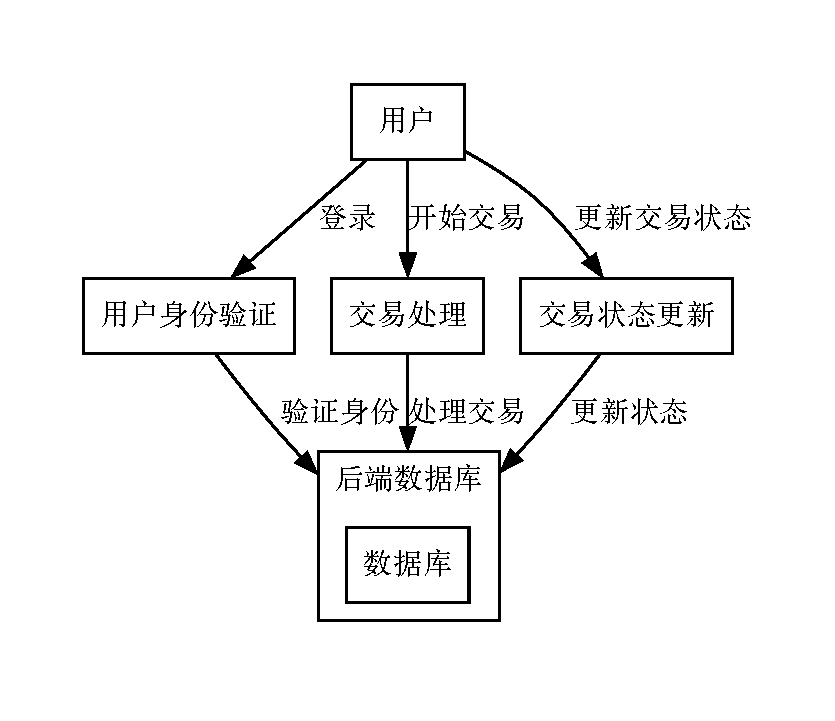
\includegraphics[width=\textwidth]{assets/onlinebanking.pdf}
\end{figure}

\subsubsection{支付结算系统}

该系统处理各种电子支付交易,如银行卡支付、电子转账、手机支付等。业务逻辑包括处理支付请求、验证用户资格、执行支付交易,然后更新账户余额和交易状态

\subsubsection{证券交易系统}

这个系统主要处理股票购买、出售和查询等功能。业务逻辑包括处理交易请求、验证用户证券账户、执行交易操作,然后在交易完成后更新用户的证券账户和持仓信息

\subsubsection{柜员业务系统}

这个系统主要用于银行网点柜员进行上台操作。需要处理各种业务,如现金存取款、转账、结售汇、贷款申请等。业务逻辑包括验证柜员的操作权限、处理柜员的业务请求,然后更新相关的账户和交易信息

\subsubsection{ERP系统}

ERP系统是用于协助银行进行财务管理、人力资源管理、客户关系管理和供应链管理等操作。业务逻辑上,它需要处理数据输入、数据处理和报表生成等工作

以上的所有系统都需要和数据库进行交互,可以采用\emph{Spring Boot}框架提供对MySQL数据库的底层支持,让开发人员可以编写业务逻辑代码而不必担心底层的数据库操作。同时,Spring Boot的优秀架构和丰富的生态也可以帮助开发人员进行快速开发,降低系统开发和维护的复杂性

业务逻辑上,需要处理的ODS可以提炼为\textbf{客户信息、存款信息、贷款信息、理财信息、票据、外汇}等

\section{架构设计}

\subsection{业务架构设计}

具体业务架构设计如下

\begin{figure}[H]
    \centering
    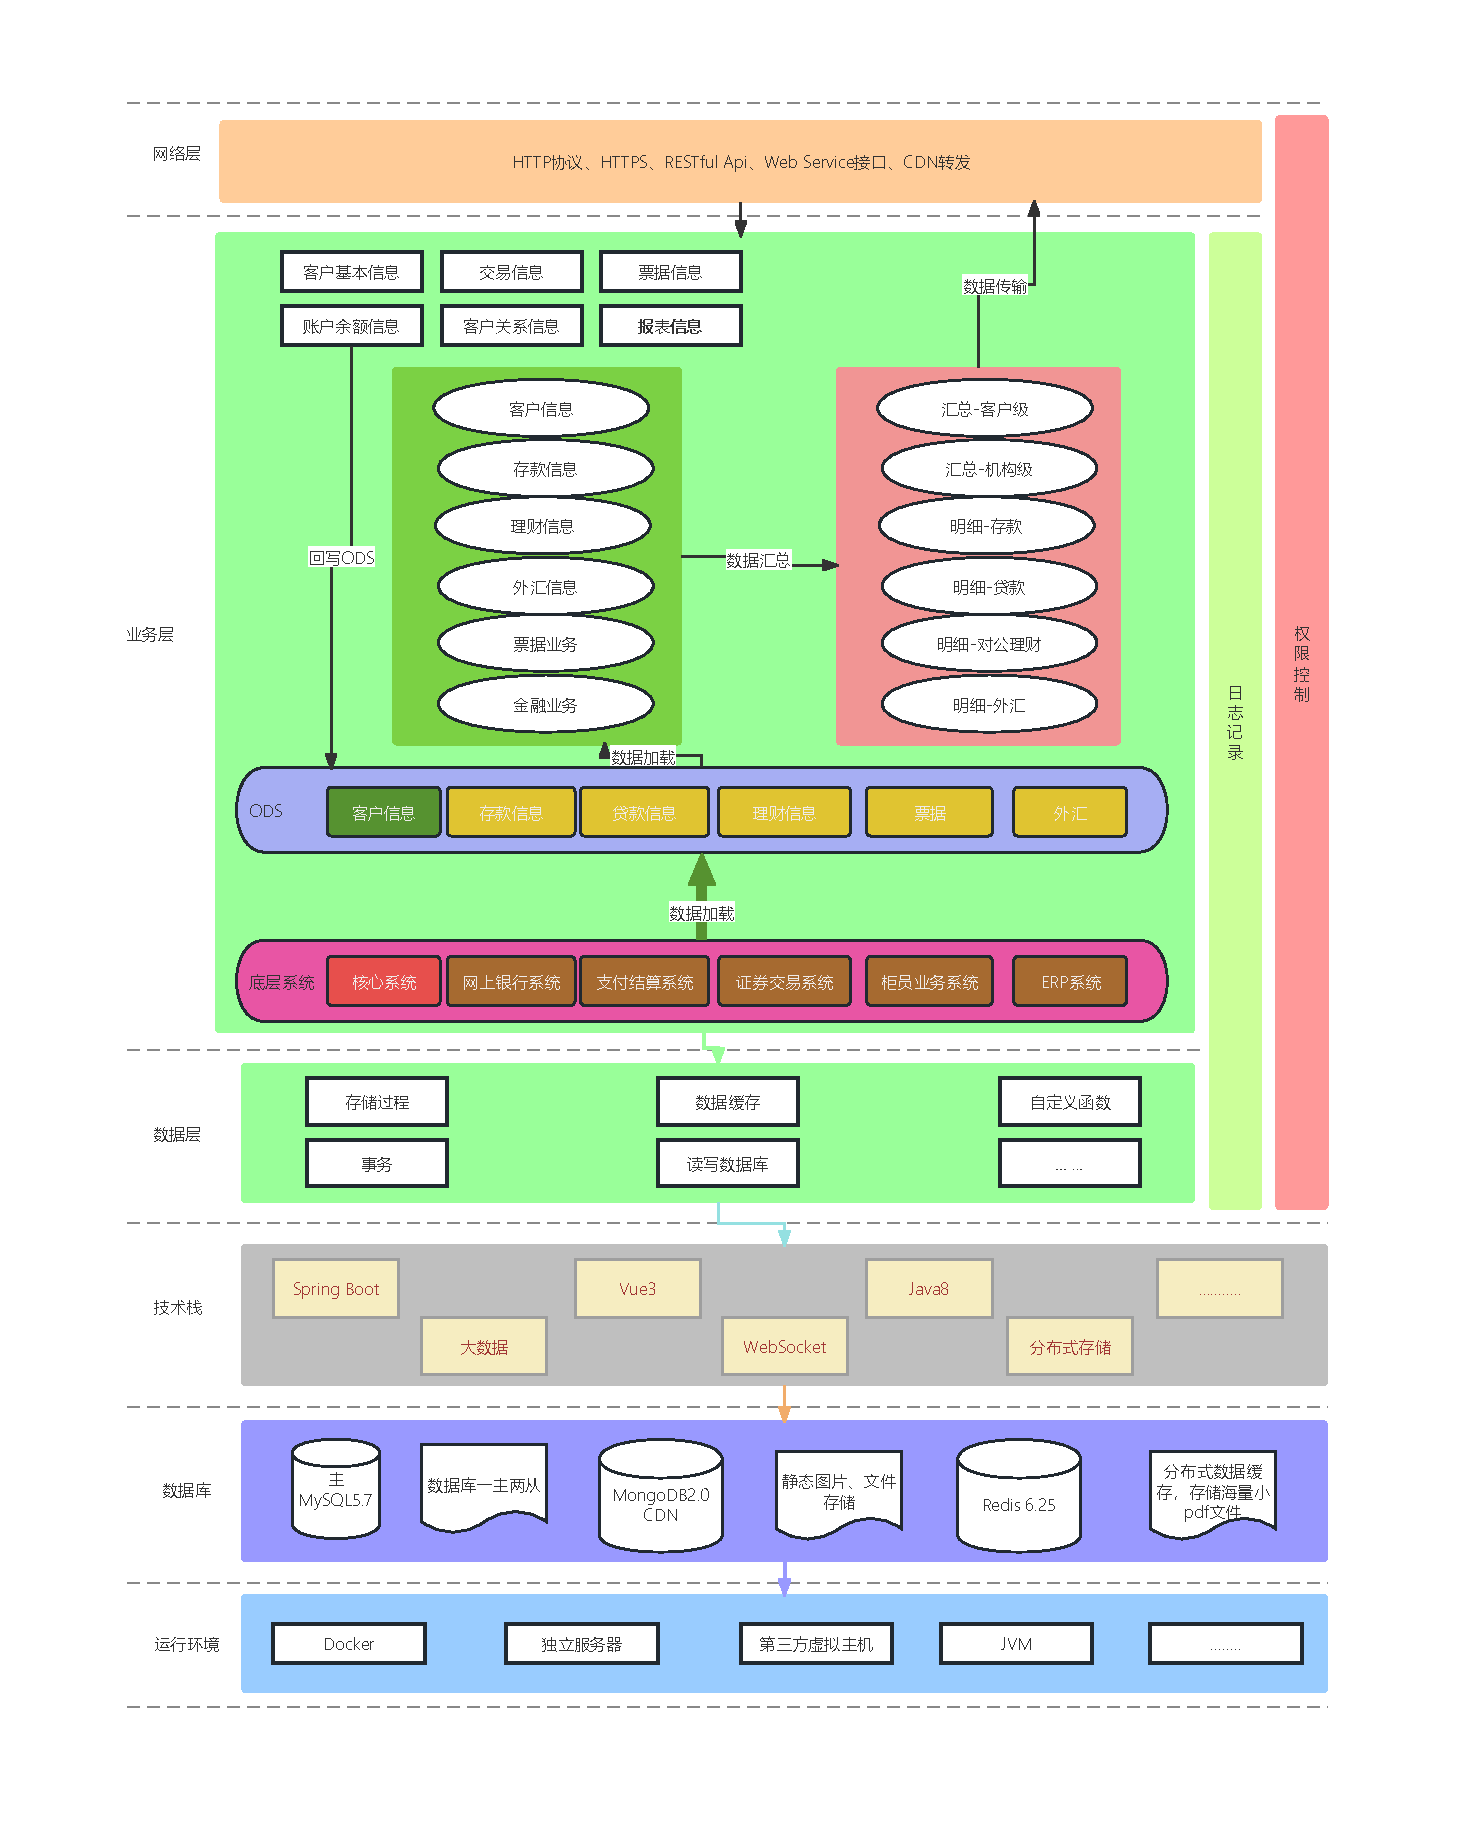
\includegraphics[width=\textwidth]{assets/系统架构设计.pdf}
\end{figure}

\end{document}